\documentclass[a4paper,twoside]{ctexart}
\usepackage{geometry}
\geometry{margin=1cm,vmargin={0pt,1cm}}
\setlength{\topmargin}{-2cm}
\setlength{\paperheight}{23cm}
\setlength{\paperwidth}{18cm}
\setlength{\textheight}{19.6cm}
\setlength{\textwidth}{15cm}
\usepackage{makecell}
\usepackage{fancyhdr}
\usepackage{siunitx}
\usepackage{amssymb}
\usepackage{indentfirst}
\setlength{\parindent}{0.5em}

\pagenumbering{arabic}

% useful packages.
\usepackage{multirow}
\usepackage{caption}
\usepackage{mathrsfs}
\usepackage{amsfonts}
\usepackage{amsmath}
\usepackage{amsthm}
\usepackage{enumerate}
\usepackage{xcolor,graphicx,float,subfigure}
\usepackage{epstopdf}
\usepackage{multicol}
\usepackage{fancyhdr}
\usepackage{layout}
\usepackage{listings}
\lstset{language=Matlab}
\lstset{breaklines}
\lstset{extendedchars=false}
\usepackage[colorlinks,linkcolor=blue]{hyperref}
\usepackage{xcolor}
\usepackage{cite}
\usepackage[numbers,sort&compress]{natbib} 
\setcitestyle{open={},close={}}
%\usepackage{natbibspacing}
%\renewcommand{\refname}{}
\usepackage{anyfontsize}


% some common command
\newcommand{\dif}{\mathrm{d}}
\newcommand{\avg}[1]{\left\langle #1 \right\rangle}
\newcommand{\pdfrac}[2]{\frac{\partial #1}{\partial #2}}
\newcommand{\op}{\odot}
\newcommand{\Eabs}{E_{\mathrm{abs}}}
\newcommand{\Erel}{E_{\mathrm{rel}}}
\newcommand{\Ediv}{\mathrm{div}}%\div是除号
\newcommand{\lrq}[1]{\left( #1 \right)}
\newcommand{\avint}[1]{\frac{1}{\left|#1\right|}\int_{#1}}

\newcommand{\upcite}[1]{\textsuperscript{\textsuperscript{\cite{#1}}}} 

\makeatletter
\newcommand\sixteen{\@setfontsize\sixteen{17pt}{6}}
\renewcommand{\maketitle}{\bgroup\setlength{\parindent}{0pt}
\begin{flushleft}
\sixteen\bfseries \@title
\medskip
\end{flushleft}
\textit{\@author}
\egroup}
\makeatother

\CTEXsetup[format={\Large\bfseries}]{section}

\title{MARS2D 测试文档}


\begin{document}
\maketitle

以下两个测试都是针对 Cubic MARS 方法的即殷集边界是用三次样条曲线表示的。测试中首先在某一个圆上均匀取点,之后由这些点生成的三次样条曲线作为初值。$h_L$取值为两个初值点间弧长的$2$倍。
\section{Vortex shear of a circular disk}
速度场如下:
\begin{equation}
  \left\{
  \begin{array}{l}
    u_x=\cos\left(\pi \dfrac{t}{T}\right)\sin^2(\pi x)\sin(2\pi y);\\
    u_y=-\cos\left(\pi \dfrac{t}{T}\right)\sin(2\pi x)\sin^2(\pi y).
  \end{array}
  \right.
\end{equation}  

测试所用参数如表\ref{tab:vortex1}所示。
\begin{table}[htbp]
    \centering\begin{tabular}{c|c}
        \hline
        参数&值\\
        \hline
        周期&$T=8$\\
        中心点&$C=(0.5,0.75)$\\
        半径&$R=0.15$\\
        $r_{\mathrm{tiny}}$&$r_{\mathrm{tiny}}=0.01$\\
        初值点数&$n=64,128,256$\\
        时间步长&$k=0.04,0.02,0.01$\\
        \hline
    \end{tabular}
    \caption{Vortex shear: 参数表}
    \label{tab:vortex1}
\end{table}

测试结果如表\ref{tab:vortex2}所示,所用误差范数$\|\mathrm{E}\|_1$是用计算出的三次样条曲线和用准确解正圆上的点生成的三次样条曲线求内部区域间近似异或面积得出的。发现可以测得四阶以上的收敛阶。

\begin{table}[htbp]
    \centering\begin{tabular}{c|ccccc}
        \hline
        $h_L=4\pi/n$&$n=64$&ratio&128&ratio&256\\
        \hline
        $\|\mathrm{E}\|_1$&4.80e-5&4.25&2.52e-6&4.97&8.06e-8\\
        \hline
    \end{tabular}
    \caption{Vortex shear: 误差及收敛阶}
    \label{tab:vortex2}
\end{table}

中间步的计算结果图如图\ref{fig:vortex}所示。

\begin{figure}[h]
	\centering  %图片全局居中
	\subfigure[$t=0$]{
		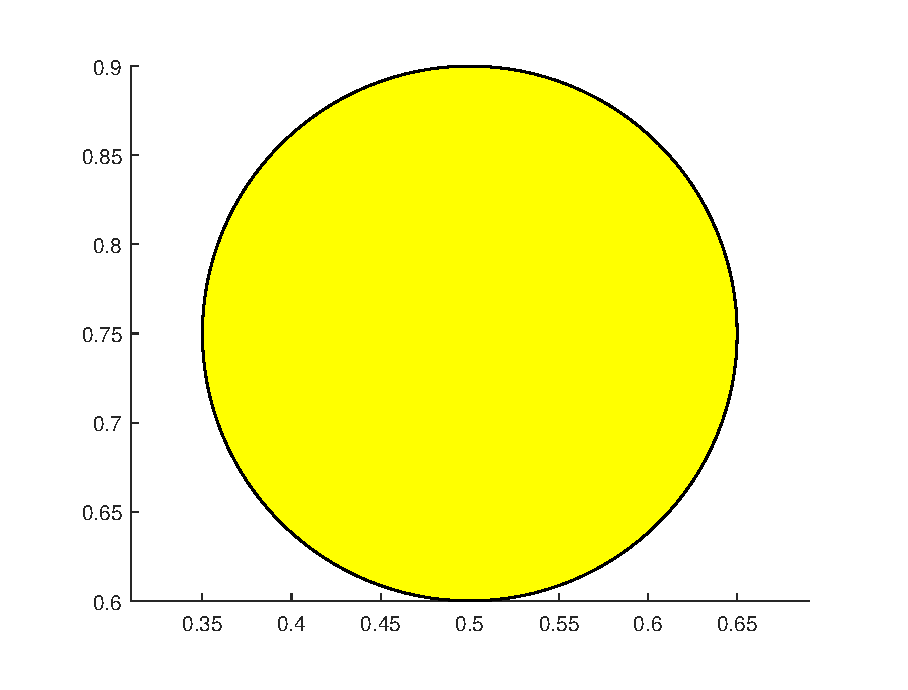
\includegraphics[width=0.3\linewidth]{vortex0T.eps}
    }
	\subfigure[$t=\dfrac{1}{8}T$]{
		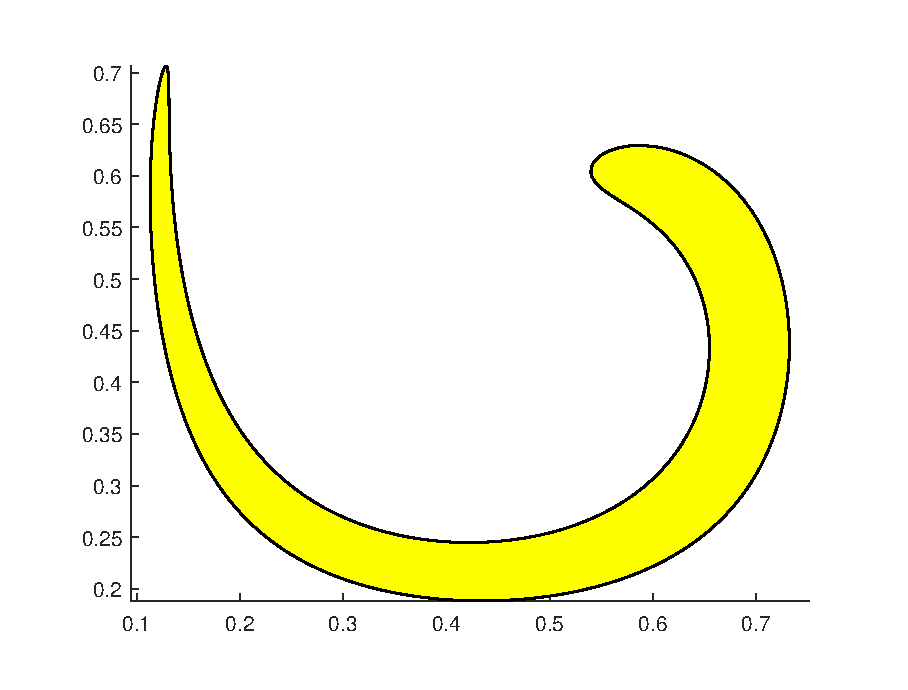
\includegraphics[width=0.3\linewidth]{vortex1_8T.eps}
    }
    \subfigure[$t=\dfrac{1}{4}T$]{
        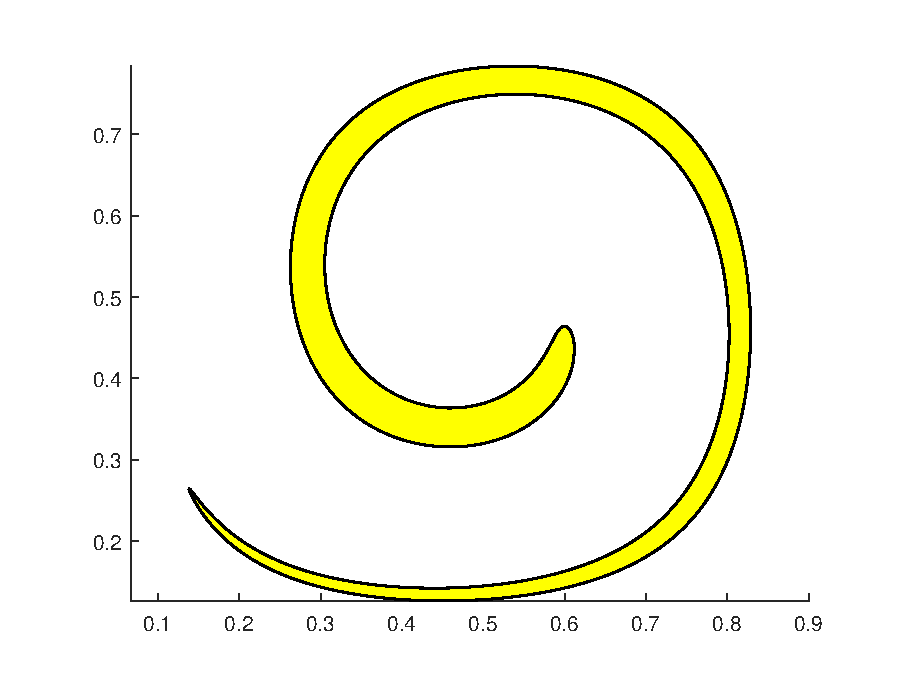
\includegraphics[width=0.3\linewidth]{vortex2_8T.eps}
    }\\
    \subfigure[$t=\dfrac{3}{8}T$]{
		\includegraphics[width=0.3\linewidth]{vortex3_8T.eps}
    }
	\subfigure[$t=\dfrac{1}{2}T$]{
		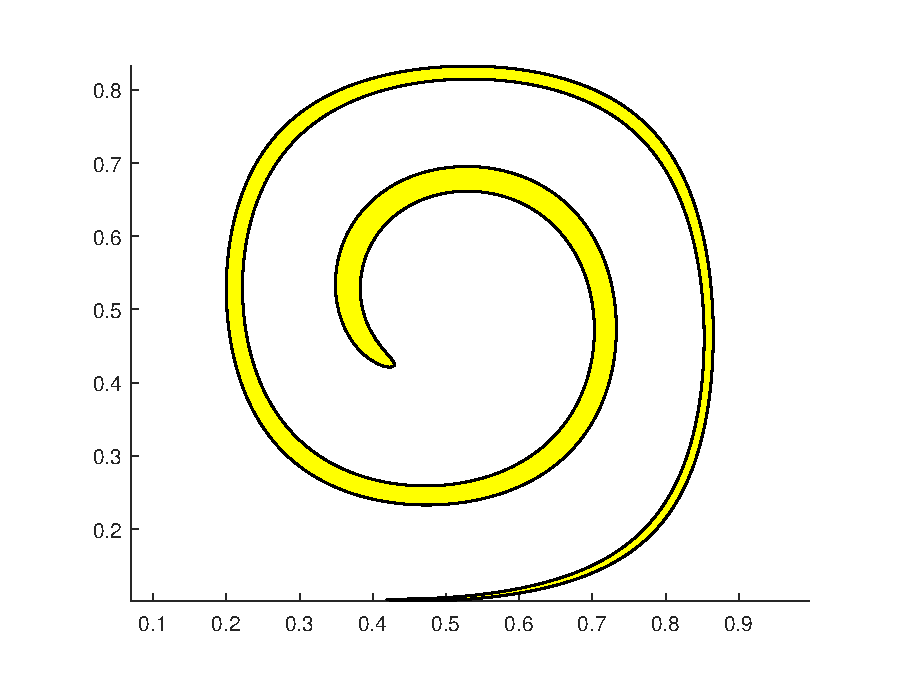
\includegraphics[width=0.3\linewidth]{vortex4_8T.eps}
    }
    \subfigure[$t=\dfrac{5}{8}T$]{
        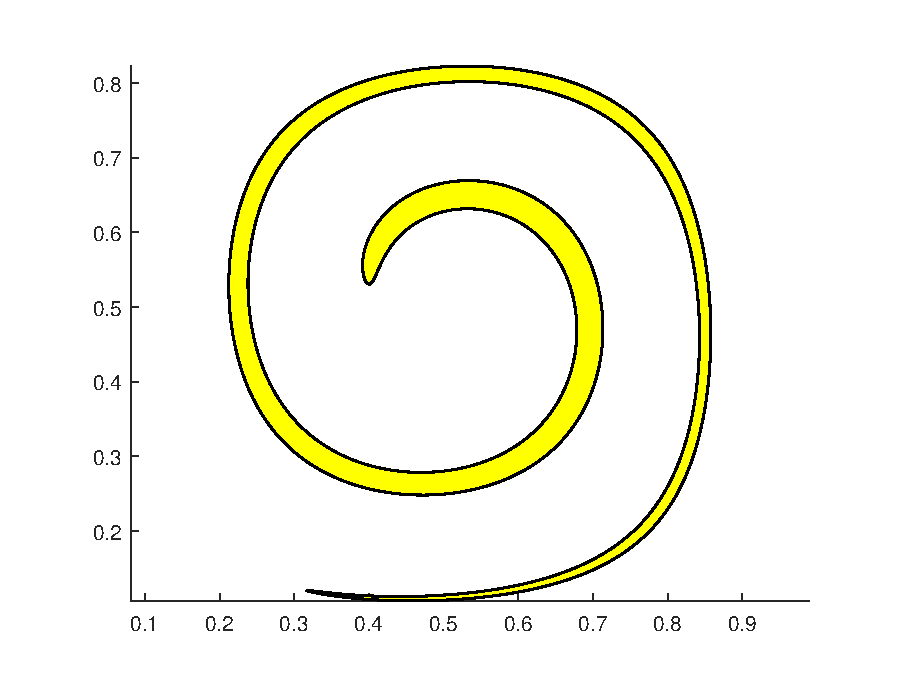
\includegraphics[width=0.3\linewidth]{vortex5_8T.eps}
    }\\
    \subfigure[$t=\dfrac{3}{4}T$]{
		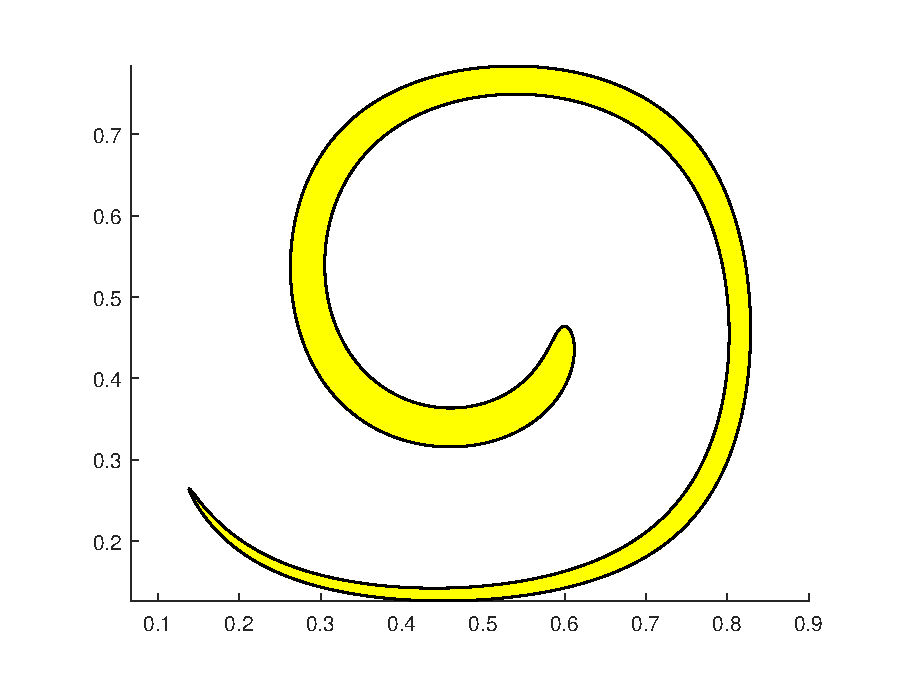
\includegraphics[width=0.3\linewidth]{vortex6_8T.eps}
    }
	\subfigure[$t=\dfrac{7}{8}T$]{
		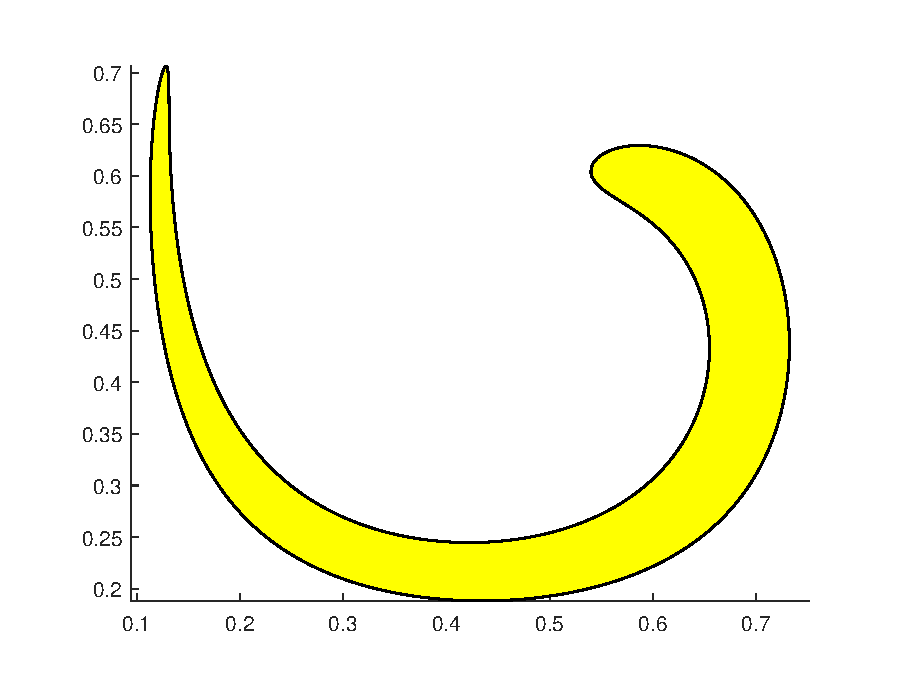
\includegraphics[width=0.3\linewidth]{vortex7_8T.eps}
    }
    \subfigure[$t=T$]{
        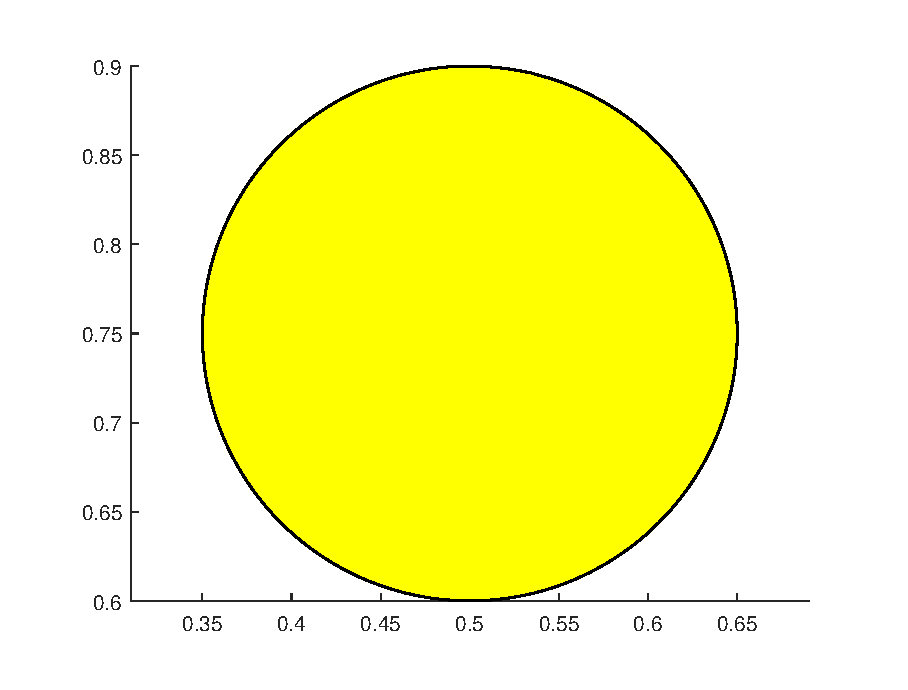
\includegraphics[width=0.3\linewidth]{vortex1T.eps}
    }
    \caption{Vortex shear: 中间步计算结果图,所用参数为 $n=128$,$k=0.02$,$r_\mathrm{tiny}=0.01$。}
    \label{fig:vortex}
\end{figure}

\section{Deformation of a circular disk}

速度场如下:
\begin{equation}
  \left\{
    \begin{array}{l}
      u_x=\cos\left(\pi \dfrac{t}{T}\right)\sin(n\pi(x+0.5))\sin(n\pi(y+0.5));\\
      u_y=\cos\left(\pi \dfrac{t}{T}\right)\cos(n\pi(x+0.5))\cos(n\pi(y+0.5));\\
      n=4.
    \end{array}
  \right.
\end{equation}

测试所用参数如表\ref{tab:deformation1}所示。
\begin{table}[htbp]
    \centering\begin{tabular}{c|c}
        \hline
        参数&值\\
        \hline
        周期&$T=2$\\
        中心点&$C=(0.5,0.5)$\\
        半径&$R=0.15$\\
        $r_{\mathrm{tiny}}$&$r_{\mathrm{tiny}}=0.01$\\
        初值点数&$n=128,256,512$\\
        时间步长&$k=0.04,0.02,0.01$\\
        \hline
    \end{tabular}
    \caption{Deformation: 参数表}
    \label{tab:deformation1}
\end{table}

测试结果如表\ref{tab:deformation2}所示,所用误差范数$\|\mathrm{E}\|_1$是用计算出的三次样条曲线和用准确解正圆上的点生成的三次样条曲线求内部区域间近似异或面积得出的。发现可以测得四阶以上的收敛阶。

\begin{table}[htbp]
    \centering\begin{tabular}{c|ccccc}
        \hline
        $h_L=4\pi/n$&$n=128$&ratio&256&ratio&512\\
        \hline
        $\|\mathrm{E}\|_1$&5.65e-5&4.61&2.31e-6&5.10&6.75e-8\\
        \hline
    \end{tabular}
    \caption{Deformation: 误差及收敛阶}
    \label{tab:deformation2}
\end{table}

中间步的计算结果图如图\ref{fig:deformation}所示。
\begin{figure}[h]
	\centering  %图片全局居中
	\subfigure[$t=0$]{
		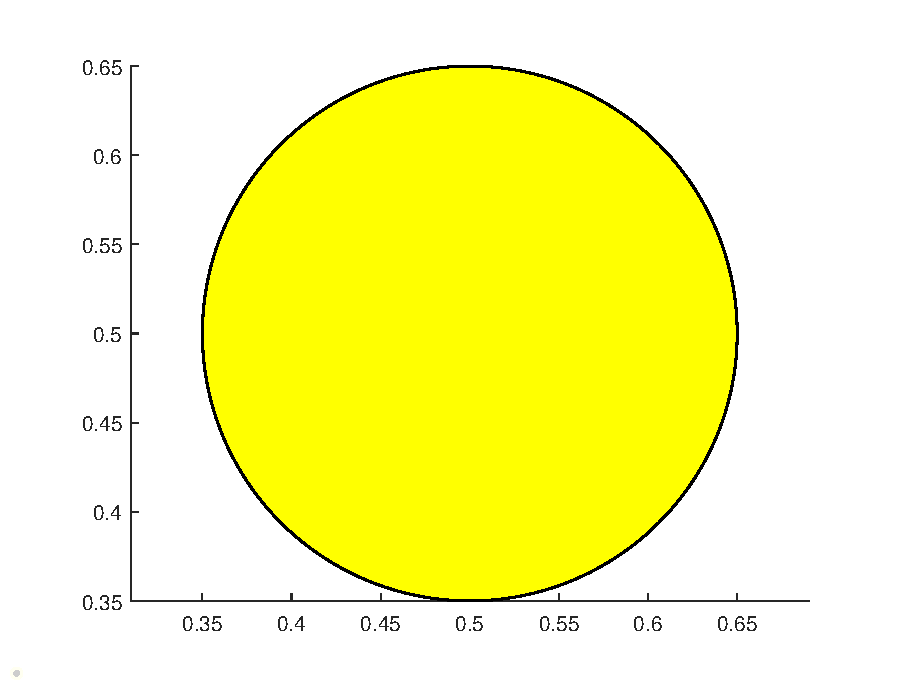
\includegraphics[width=0.3\linewidth]{deformation0T.eps}
    }
	\subfigure[$t=\dfrac{1}{8}T$]{
		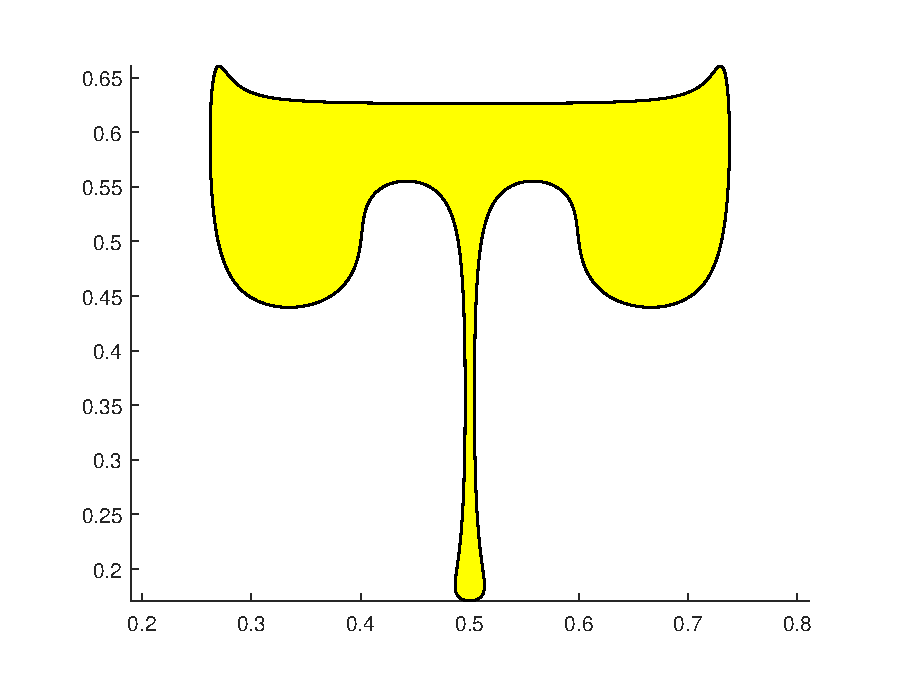
\includegraphics[width=0.3\linewidth]{deformation1_8T.eps}
    }
    \subfigure[$t=\dfrac{1}{4}T$]{
        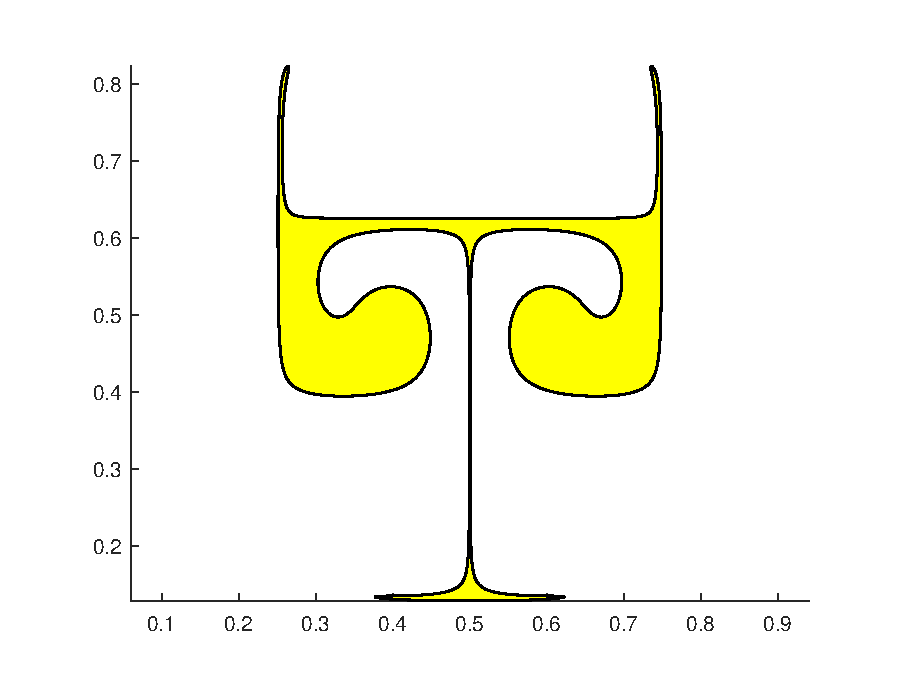
\includegraphics[width=0.3\linewidth]{deformation2_8T.eps}
    }\\
    \subfigure[$t=\dfrac{3}{8}T$]{
		\includegraphics[width=0.3\linewidth]{deformation3_8T.eps}
    }
	\subfigure[$t=\dfrac{1}{2}T$]{
		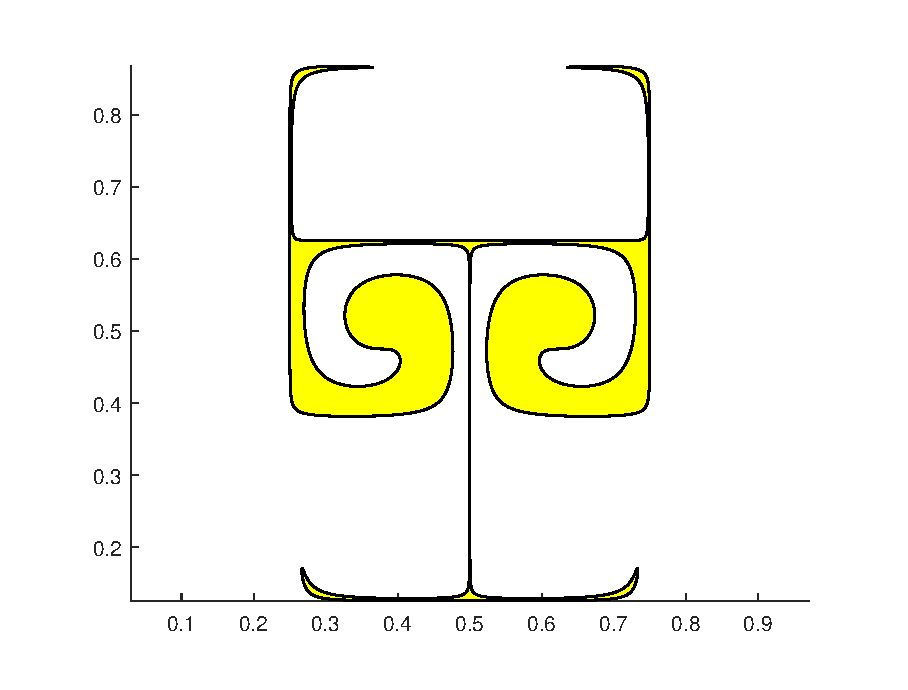
\includegraphics[width=0.3\linewidth]{deformation4_8T.eps}
    }
    \subfigure[$t=\dfrac{5}{8}T$]{
        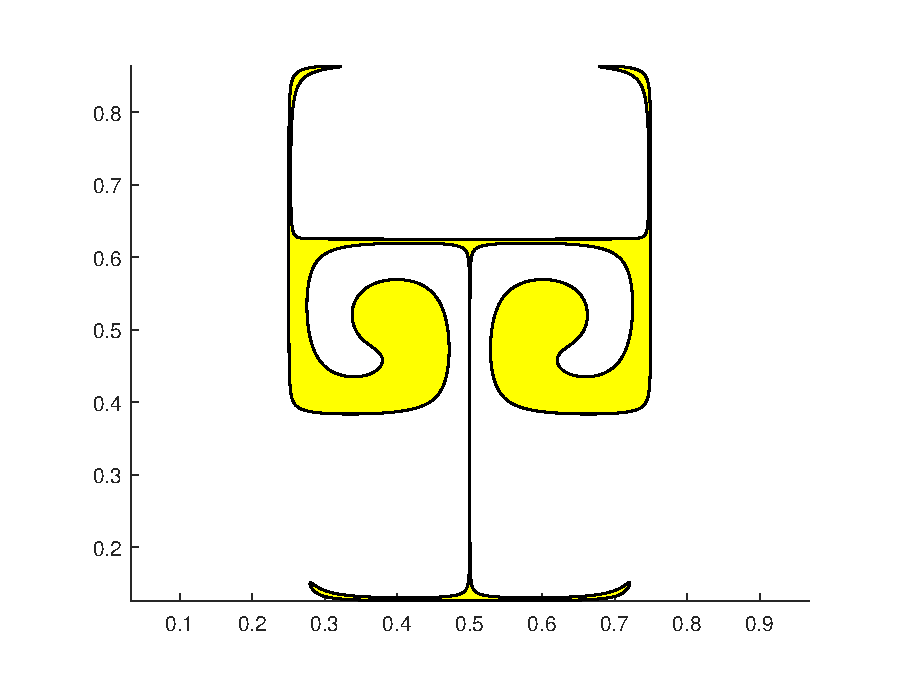
\includegraphics[width=0.3\linewidth]{deformation5_8T.eps}
    }\\
    \subfigure[$t=\dfrac{3}{4}T$]{
		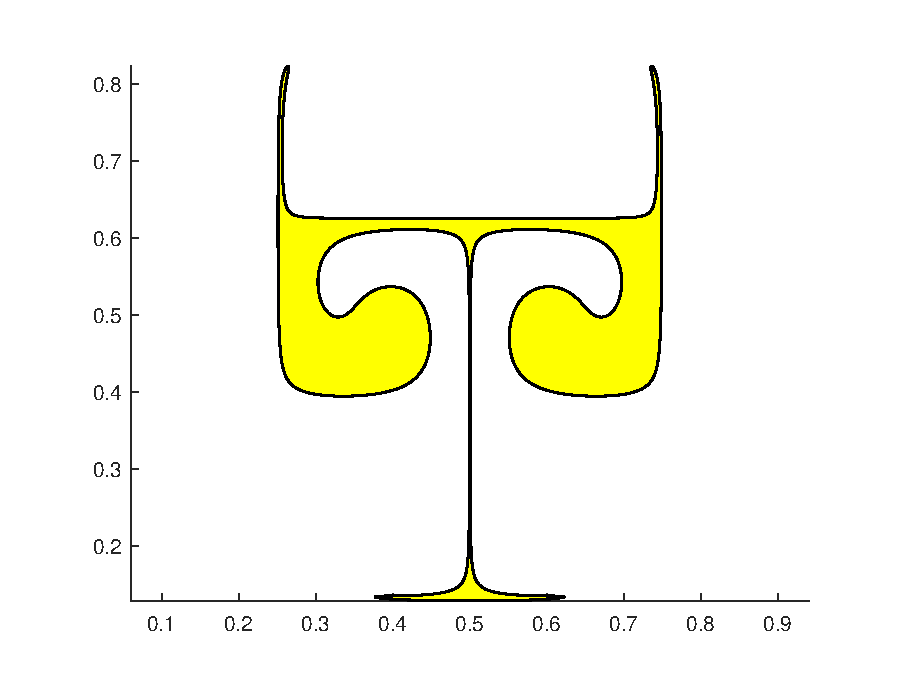
\includegraphics[width=0.3\linewidth]{deformation6_8T.eps}
    }
	\subfigure[$t=\dfrac{7}{8}T$]{
		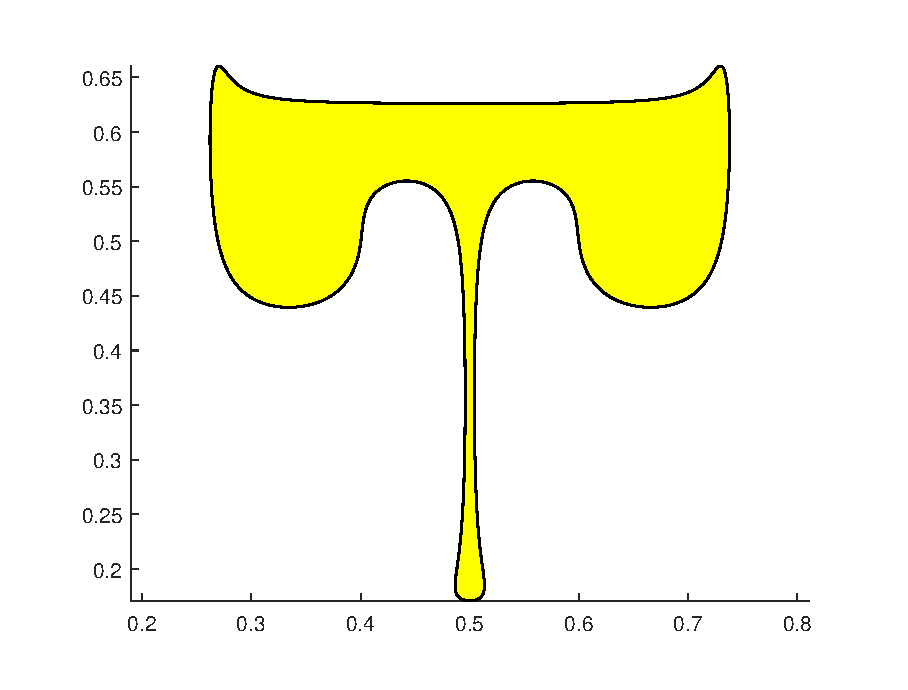
\includegraphics[width=0.3\linewidth]{deformation7_8T.eps}
    }
    \subfigure[$t=T$]{
        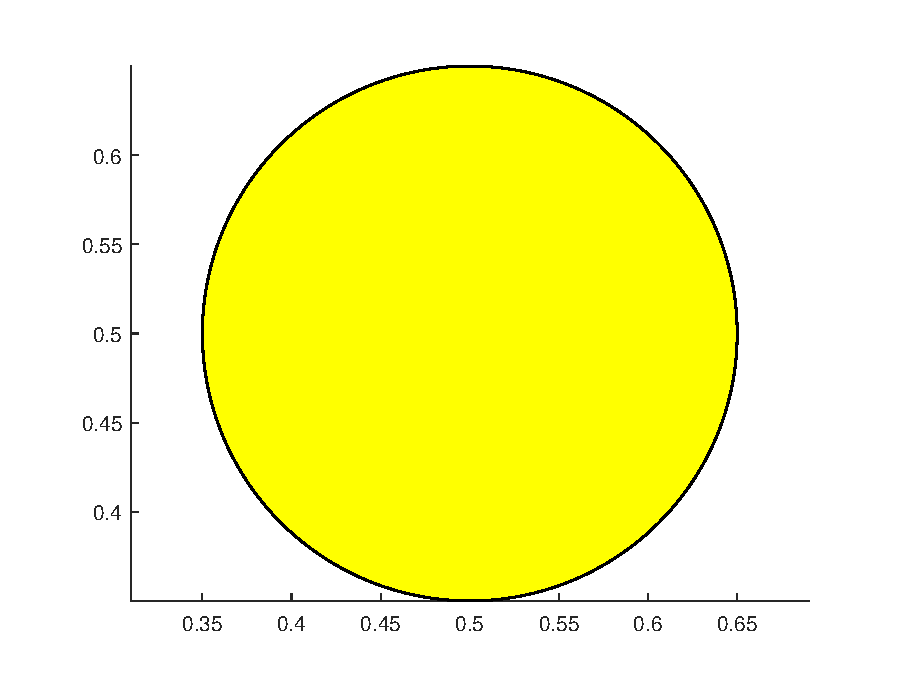
\includegraphics[width=0.3\linewidth]{deformation1T.eps}
    }
    \caption{Deformation: 中间步计算结果图,所用参数为 $n=256$,$k=0.02$,$r_\mathrm{tiny}=0.01$。}
    \label{fig:deformation}
\end{figure}

\end{document}